\documentclass{article}

\title{Math 3010 Midterm 2 "Cheat Sheet"}
\author{Lincoln Sand}

\usepackage{amsfonts}
\usepackage{graphicx}
\usepackage{amssymb}
\usepackage{amsmath}
\usepackage{listings}
\usepackage{hyperref}


\DeclareMathOperator{\sech}{sech}
\newcommand{\NN}{\mathbb{N}}
\newcommand{\RR}{\mathbb{R}}
\newcommand{\QQ}{\mathbb{Q}}
\newcommand{\ZZ}{\mathbb{Z}}
\newcommand{\dV}{\;\mathrm{d}V}
\newcommand{\dA}{\;\mathrm{d}A}
\newcommand{\dx}{\;\mathrm{d}x}
\newcommand{\dy}{\;\mathrm{d}y}
\newcommand{\dz}{\;\mathrm{d}z}
\newcommand{\cA}{\mathcal{A}}
\newcommand{\Bb}{\mathcal{B}}
\newcommand{\Ww}{\mathcal{W}}
\newcommand{\Dd}{\mathcal{D}}
\newcommand{\Ss}{\mathcal{S}}
\newcommand{\Ee}{\mathcal{E}}
\DeclareMathOperator{\im}{im}

\usepackage{blindtext}
\usepackage{geometry}
\geometry{
a4paper,
total={170mm,257mm},
left=20mm,
top=20mm,
}

\begin{document}

Math 3010 Midterm 2 "Cheat Sheet"

Lincoln Sand

- Historical Data:

* al-Khwarizimi; 830 Baghdad; Decimal arith., linear and quadratic alg. eqns.

* Bhaskara II; 1150 Ujjian; Solved Pell's equation using the cyclic process.

* Brahmagupta; 650 Bhinmal; Quadratic eqns., composition formula for Pell's eqn.

* Cardano; 1545 Bologna; First published solution of cubic eqns.

* Descartes; 1637 Holland; Used coords to relate curves to solutions of eqns.

* Desargues; 1639 Paris; Projective geometry

* Leonardo; 1202 Pisa; Introduced Hindu-Arabic notation and algebra to Europe.

* Zhang Cang; 150 BC Chang'an; 246 problems in proportions, $3 \times 3$ systems.

* Ptolemy; 145 Alexandria; Astronomy and trig of geocentric universe.

* Qin Juishao; 1247 Hangzhou; Chinese Remainder Theorem, polynomial eqns.

* Copernicus; 1543 Frauenberg; Planet orbits around sun generated by epicycles.

* Kepler; 1609 Prague; Planets orbit sun on elliptical paths of different speeds.

* Lui Hui; 263 Shansi Province; Standard text on systems of eqns and measuring.

* Napier; 1614 Merchison; Tables of logarithms and instructions for their use.

* Viete; 1591 Paris; Solved cubic eqns. using trig identities.

* Archimedes (287 - 212 BC Syracuse);; Apollonius (250 - 175 BC Alexandria);; Heron (25 - 105 AD Alexandria);; Hipparchus (190 - 120 BC Bithynia);; Ptolemy (100 - 178 AD Alexandria) 

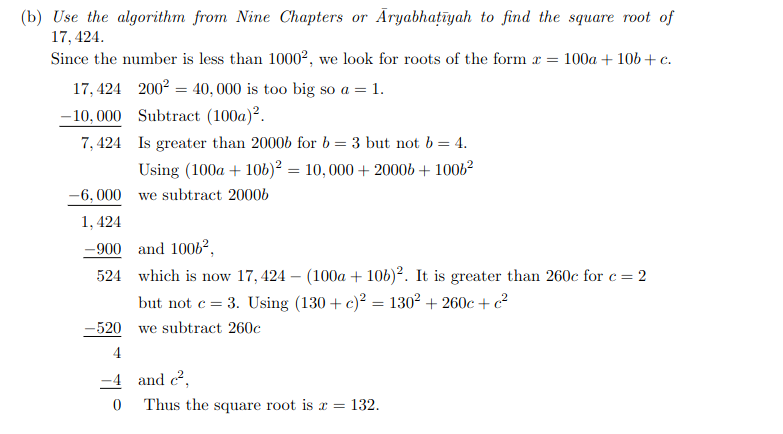
\includegraphics[width=\linewidth]{square_root_algorithm}


Brahmagupta's identity:

For given $n$, the product of two numbers of the form $a^2 + n b^2$
is itself a number of that form. Specifically,
\[(a^2 + n b^2) \cdot (c^2 + n d^2) = (a c - n b d)^2 + n(a d + b c)^2
= (a c + n b d)^2 + n(a d - b c)^2\]

Fermat's Little Theorem: $a^{p-1} \equiv 1 (\text{mod p})$.

Chinese Remainder Theorem:

Given $x = a_i \, (\text{mod $m_i$})$,
compute $M = m_1 \cdot m_2 \dots m_n$,
and for each $i$, compute $M_i = \frac{M}{m_i}$.

Compute the multiplicative inverses such that $M_i \cdot M_i^{-1} = 1 \, (\text{mod $m_i$})$.

The solution is given by $x = \sum_{i=1}^n a_i \cdot M_i \cdot M_i^{-1} (\text{mod M})$.

Heron's triangle area: $A^2 = s(s-a)(s-b)(s-c)$.

Hipparchus supplementary angle and half-angle formulas for chords:
\[\text{crd}^2(180^\circ - \beta) = 4 R^2 - \text{crd}^2(\beta)\]
\[\text{crd}^2(\beta/2) = R(2 R - \text{crd}(180^\circ - \beta))\]

Theorem: Let $A$, $B$, $C$, and $D$ be four points in order on the circle. Then the
lengths of sides and diagonals of the quadrilateral $ABCD$ satisfy the equation:
$AB \cdot CD + BC \cdot DA = AC \cdot BD$


Archimedes used a marked straightedge to trisect an angle.



Ptolemy's difference formula for chords:

$2 R \cdot \text{crd}(\beta - \mu) = \text{crd}(\beta) \cdot \text{crd}(180^\circ - \mu) - \text{crd}(\mu) \cdot \text{crd}(180^\circ - \beta)$


Liu Hui's method to approximate $\pi$:

1. Start with hexagon, $P_6 = 6 \cdot 1 = 6$.

2. Doubling number of sides to get dodecagon.

3. Calculate the side length of the dodecagon: For a hexagon inscribed in a unit circle, each triangle formed by two adjacent vertices and the center of the circle is an equilateral triangle. If we add a perpendicular line from the center to the midpoint of one side, we divide the equilateral triangle into two 30-60-90 right triangles.

$s_{12} = \sqrt{1^2 - \left(\frac{1}{2}\right)^2} = \sqrt{\frac{3}{4}} = \frac{\sqrt{3}}{2}$.

The side length of the dodecagon is half the side length of the hexagon due to the properties of a 30-60-90 triangle.

$P{12} = 12 \cdot s_{12} = 6 \sqrt{3}$

This is an approximation for the unit circle circumference, which is $2 \pi$,
thus, $\pi \approx 3 \sqrt{3}$.

Sum of geometric series: $S = \frac{a(1 - r^n)}{1-r}$.
If $|r| < 1$, then it converges to: $S = \frac{a}{1-r}$.

- Euclidean GCD algorithm/diophantine example:

Find $x, y \in \ZZ$ such that $gcd(198, 168) = 198x + 168y$.

\[198 = 1 \cdot 168 + 30; 168 = 5 \cdot 30 + 18; 30 = 1 \cdot 18 + 12;\]
\[18 = 1 \cdot 12 + 6; 12 = 2 \cdot 6 + 0\]
So, $gcd(198, 168) = 6$.

\[6 = 18 - 12 = 18 - (30 - 18) = 2 \cdot 18 - 30 = 2 \cdot (168 - 5 \cdot 30) - 30\]
\[= 2 \cdot 168 - 11 \cdot 30 = 2 \cdot 168 - 11 \cdot (198 - 168) = 13 \cdot 168 - 11 \cdot 198\]
So, $x = -11, y = 13$.


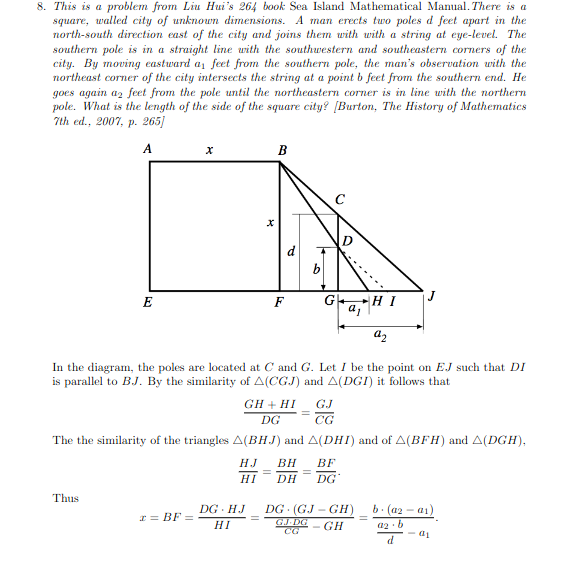
\includegraphics[width=150mm]{walled_city}


\end{document}
